\documentclass[a4paper, 11pt] {article}
\usepackage[T1]{fontenc}
\usepackage[utf8]{inputenc}
\usepackage[english]{babel}
\usepackage{url} 
\usepackage{graphicx} 
\usepackage{hyperref} 

\begin{document}
\title{%
  Automation and Control Laboratory \\
  \large Magnetic Bearing \\
    (MAGLEV 2)}
    
\bigskip
    
\author{ 10601188 – El Moukhal Wassim \\
10610853 – Pellei Francesco \\
10581773 – Rodrigues Da Silva Nascimento Kiara Rodrigues \\
10608561 – Rizzo Alessandro\\ }

\bigskip

\date{2022-2023} 

\maketitle

\newpage

\tableofcontents
\newpage



\section{Introduction}

\subsection{Laboratory Purpose}
Our laboratory experience had the following goals:
\begin{itemize}
\item Modelling of the assigned system
\item Identification of the parameters 
\item Validation of the developed model 
\item Application of different control strategies 
\item Comparison between different control strategies 
\end{itemize} 

      

\subsection{System Description}
Magnetic Levitation technology (MagLev), uses the magnetic force generated by coils or magnets to reduce physical contact between stationary and moving parts. Due to the nature of the magnetic force, the system is unstable and highly non-linear, so an appropriate control technique is necessary to stabilise the system. \\
The system assigned to the group is composed of: 
\begin{itemize}
\item An aluminium structure 
\item Two coils in series placed on the top of the structure. Each coil has $n = 860$ windings, both connected to an electronic board that is used to inject current to generate a magnetic flux inside the ferromagnetic material 
\item A parallelepiped specimen made of ferrite, and mounted on a vertical slider that avoids any displacement of the moving element along the horizontal plane. The total mass of the specimen, considering also the clamps and the screws is $m = 0.824 kg$ and its cross-section is $A = 8.4*10^{-4} m^{2}$
\item A lasers sensor used to measure the position of the moving block with respect to the fixed structure. 
\item     PoliArd electronic board, which allows to perform real-time control logics 
\end{itemize}

Originally the system included also another couple of coils in series placed under the moving block. They could be useful to better control the system, but unfortunately this additional part is no longer available. \\

\begin{figure}
\begin{center}
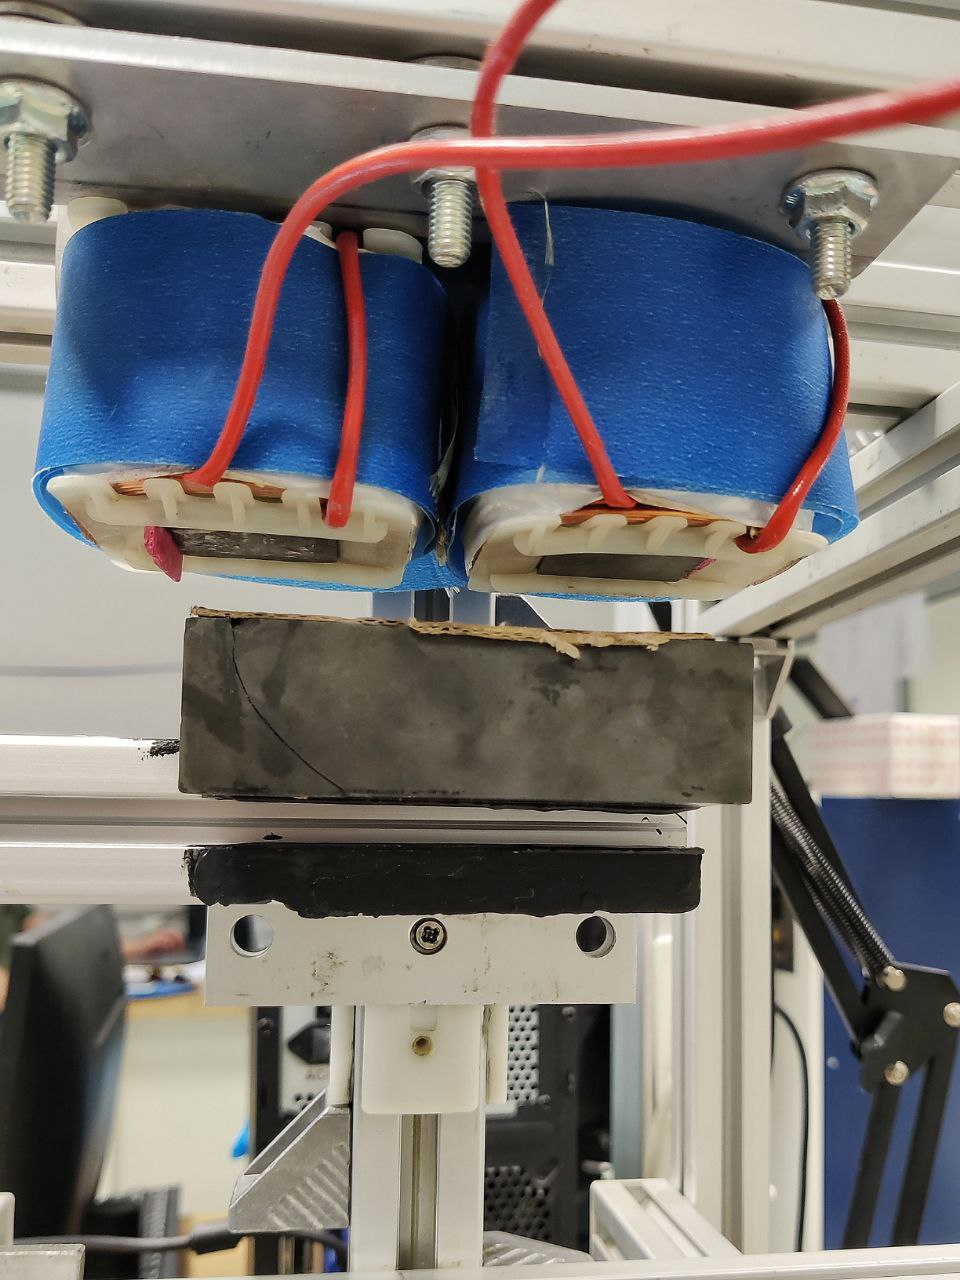
\includegraphics[scale=0.2]{Images/1_magnete}
\end{center}
\caption{Specimen and coils}
\end{figure}


\subsection{Electronic equipment and Settings}

\textbf{Finish writing in report + Poliard image + I/O scheme + simulink blocks}



\section{Electrical Model}
The following section explains the model chosen for the electrical part of the system, and the techniques used to identify its parameters.

\begin{figure}
\begin{center}
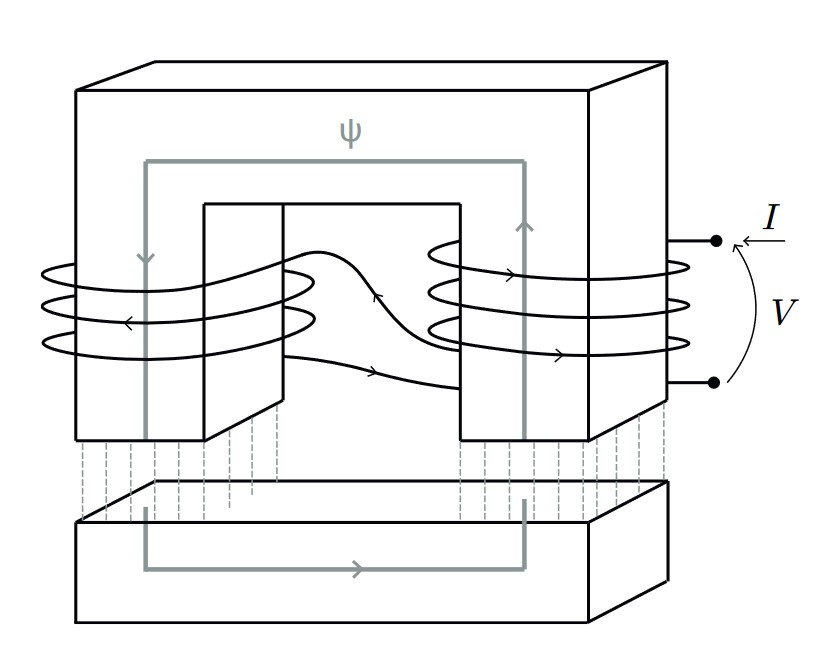
\includegraphics[scale=0.5]{Images/2_schema_elettrico}
\end{center}
\caption{MagLev representation}
\end{figure}


\subsection{System Equation}
The electrical part of the system is described by:
\begin{equation}
V = R \cdot i(t) + \frac{d(L(i(t),x) \cdot i(t)}{dt}
\end{equation}




\subsection{Parameter Identification}
 Nulla et eros odio. Aliquam at mi interdum, bibendum ipsum id, tempus erat. Quisque viverra neque ligula, eu pharetra enim dictum vel. Aliquam mattis pharetra libero ut consequat. Donec porttitor massa dolor, sit amet molestie metus ultrices at. Ut mollis tortor ac lectus luctus vulputate. Pellentesque pretium nec odio non tempus. Quisque dolor metus, mattis et tempor vitae, vulputate nec odio. Proin placerat felis justo, in placerat lorem molestie in. Vivamus efficitur lacus a lacus tempor pharetra.
\\
Pellentesque eu nibh sit amet nisl hendrerit mollis. Maecenas eget tortor vestibulum, dictum ipsum at, consectetur mauris. Aliquam sodales viverra erat, ut molestie elit efficitur sit amet. Proin nec venenatis felis, a laoreet quam. Mauris aliquet ligula in odio auctor pulvinar. Fusce porta elit ut mi ultrices imperdiet. Maecenas ac mauris sit amet erat posuere sodales ac vel nunc. Morbi porta finibus pretium. In hac habitasse platea dictumst. 


\section{Mechanical model}

Pellentesque volutpat, orci eu feugiat molestie, lacus ex sodales dui, nec rhoncus diam purus at massa. Maecenas ac odio eget justo venenatis rhoncus vel in orci. Etiam ac eros rutrum, aliquam ante nec, pharetra felis. Ut maximus elementum felis sed aliquet. Phasellus sit amet mollis tortor. Nunc et pharetra diam, eleifend efficitur urna. Sed gravida lacus et urna consequat, vulputate efficitur mi tincidunt. Integer convallis sapien dui, vitae varius tellus euismod sed. Vivamus odio diam, porttitor id laoreet at, dictum vitae leo. Suspendisse dignissim sit amet lacus ut malesuada. Quisque lobortis suscipit nisi a malesuada. Sed et libero vel dolor pretium tincidunt vitae a felis. Maecenas fermentum vehicula magna, in tristique leo scelerisque eu. Suspendisse nec blandit nunc. Suspendisse potenti. Sed posuere commodo porta. 




\section{Control}

 Integer ultrices, ante vitae euismod consectetur, tellus libero efficitur ipsum, pulvinar fermentum quam sapien quis ante. Proin a nisl sit amet magna suscipit faucibus. Nulla ut semper nibh, et accumsan quam. Integer tincidunt tellus ac tellus vulputate, in porttitor felis sagittis. Duis lacus sapien, commodo quis aliquam consectetur, fermentum elementum elit. Donec aliquet arcu at neque blandit, sed mattis massa accumsan. Vivamus tempor ligula vitae eros pharetra tristique. Quisque vestibulum ut justo id commodo. Duis facilisis mattis ipsum vitae molestie.
\\
Etiam quis dapibus elit. Sed mollis magna in risus efficitur, sit amet sagittis dui volutpat. Ut a posuere nisi, et condimentum lectus. Aenean aliquam neque quis tortor iaculis egestas. Nulla suscipit dolor sit amet fermentum maximus. Maecenas porttitor, arcu nec aliquam laoreet, libero erat facilisis diam, eget commodo nibh nulla at erat. Aenean interdum sapien neque, in accumsan elit imperdiet a. Sed faucibus condimentum odio non scelerisque. Ut risus diam, elementum eleifend ex a, volutpat fringilla arcu. 


\section{Verification}

Lorem ipsum dolor sit amet, consectetur adipiscing elit. Phasellus ac malesuada arcu. Pellentesque a volutpat mi. Pellentesque dictum dolor at nisi accumsan, at efficitur elit efficitur. Suspendisse placerat nibh sit amet dolor consectetur, convallis eleifend risus rutrum. Praesent posuere vehicula est at pretium. In tempus, ipsum eu viverra vulputate, felis neque dignissim mi, et blandit tellus tellus vehicula tortor. Etiam eu fringilla turpis. Morbi semper, ligula non dignissim convallis, diam lacus elementum dui, nec dignissim lorem lectus id ex. Vestibulum ante ipsum primis in faucibus orci luctus et ultrices posuere cubilia curae; Sed sed vulputate odio. Maecenas et erat sed ipsum condimentum interdum. Nullam sodales ligula eget sapien scelerisque lobortis. Donec euismod sem vitae justo tempus tincidunt. Proin lacinia mi a urna lacinia, et vulputate sapien convallis. 



\section{Results}


Donec consequat eros in eros facilisis hendrerit. Maecenas varius, felis commodo vehicula malesuada, felis eros suscipit dui, et suscipit sapien diam vel arcu. Mauris egestas pharetra finibus. Sed non nulla at ligula efficitur gravida sed eu sem. Suspendisse varius nisi eget arcu imperdiet tempus. Duis gravida metus quis arcu tincidunt cursus. Morbi laoreet, massa quis molestie convallis, dolor neque sagittis justo, quis fermentum ligula sem a felis. Maecenas pellentesque volutpat imperdiet. Sed mattis ipsum a felis lacinia, quis luctus risus mattis. Vestibulum lacinia ligula vitae iaculis molestie. Sed iaculis magna egestas ultricies iaculis. Nullam ut condimentum ipsum, vitae semper arcu. 




\section{Conclusion}

 Nulla et eros odio. Aliquam at mi interdum, bibendum ipsum id, tempus erat. Quisque viverra neque ligula, eu pharetra enim dictum vel. Aliquam mattis pharetra libero ut consequat. Donec porttitor massa dolor, sit amet molestie metus ultrices at. Ut mollis tortor ac lectus luctus vulputate. Pellentesque pretium nec odio non tempus. Quisque dolor metus, mattis et tempor vitae, vulputate nec odio. Proin placerat felis justo, in placerat lorem molestie in. Vivamus efficitur lacus a lacus tempor pharetra.

Pellentesque eu nibh sit amet nisl hendrerit mollis. Maecenas eget tortor vestibulum, dictum ipsum at, consectetur mauris. Aliquam sodales viverra erat, ut molestie elit efficitur sit amet. Proin nec venenatis felis, a laoreet quam. Mauris aliquet ligula in odio auctor pulvinar. Fusce porta elit ut mi ultrices imperdiet. Maecenas ac mauris sit amet erat posuere sodales ac vel nunc. Morbi porta finibus pretium. In hac habitasse platea dictumst. 

\section*{Sources and citations}




\end{document}